% !TeX spellcheck = es_ES
\documentclass[arial,a4paper,print]{article}

\usepackage{amsmath}
\usepackage{helvet}
\usepackage{lipsum}
\usepackage{multirow}
\usepackage{array}
\usepackage{physics}
\usepackage[version=4]{mhchem}
\usepackage{epsfig}
\usepackage{amssymb}
%\usepackage{svrsymbols}
\usepackage{siunitx}
\usepackage{graphicx}
\usepackage{cancel}
\usepackage{float}
\usepackage{subcaption}
\usepackage[labelfont=sc, font={footnotesize, singlespacing}]{caption}
\usepackage[margin=2cm]{geometry}  

\renewcommand{\familydefault}{\sfdefault}

\usepackage[spanish]{babel}
%opening
\title{Química: Selectividad 2022}
\author{tomiock}

\begin{document}
	
\maketitle
	
\section{La radiación, los átomos y las moléculas}
\subsection{Radiación EM y interacciones entre átomos}
La radiación electromagnética se puede caracterizar mediante diversas magnitudes: 
\begin{enumerate}
	\item Longitud de onda ($\lambda$): \\
	Distancia mínima entre dos puntos en fase (mismo estado de vibración. 
	\item Periodo ($T$): \\
	El tiempo que tarda la onda en recorrer la longitud de onda. 
	\item Frecuencia ($\nu$): \\
	El número de longitudes de onda que pasan por un punto determinado en un segundo. Se puede relacionar con su longitud de onda y velocidad de propagación: 
	\begin{equation*}
			\nu = \frac{c}{\lambda}
	\end{equation*}
	En el caso de la radiación EM su velocidad de propagación es $c$, la velocidad de la luz, claro. 
\end{enumerate}
	
Se relacionan la energía con la longitud de onda y la frecuencia de la siguiente manera:
	\begin{equation*}
		E = h\frac{c}{\lambda} 
	\end{equation*}
	
\subsubsection{Radiación Infrarroja}
Los fotones ubicados en el espectro infrarrojo no tienen suficiente energía para poder provocar la transición electrónica de los átomos, pero si que los hacen vibrar. Cuando la radiación infrarroja es absorbida por los átomos estos usualmente pases de un estado de vibración a otro más energético, empiezan a vibrar de otra manera. Pueden o no pasar a un estado de vibración excitado. Más adelante veremos como se utiliza este fenómeno para determinar los grupos funcionales de substancias. 
	
\subsubsection{Espectro Visible}
En cambio cuando se absorben los fotones ubicados en el espectro visible, estos provocan saltos electrónicos, cuando un electrón pasa a estar en un orbital diferente con más energía.


Además conviene saber cuál es la relación entre la radiación IR y UV con el efecto invernadero y la capa de ozono.  
	
	
\subsection{Modelo atómico, Propiedades Periódicas de los Elementos y Cuantificación de la Energía} 

\subsubsection{Hipótesis de Planck}
La energía va en paquetes, osea cuantos de energía, de ahí viene la palabra cuántica, lo pillas?

También piensa en esta ecuación:
\begin{equation*}
	E = h\nu
\end{equation*}

No tengo nada más que decir.

\subsubsection{Modelos de los átomos}
Hay una nube de probabilidades a la cual llamamos orbital. Hay varios tipos de orbitales que están organizados según la energía que tienen. Hay que recortad que están organizados discretamente, no hablamos de un intervalo continuo de energía. 

Los orbitales se describen a partir de los números cuánticos asociados a un elemento:
\begin{enumerate}
\item N. Cuántico Principal $n$:\\
Describe lo grande que es un orbital. Es un número natural (sin cero), $n\in\mathbb{N}$. 

\item N.C. Secundario $l$:\\
Describe la forma del orbital, puede tener 4 valores:
\begin{align*}
	l = 0 \rightarrow \text{orbital } s \\
	l = 1 \rightarrow \text{orbital } p \\
	l = 2 \rightarrow \text{orbital } d \\
	l = 3 \rightarrow \text{orbital } f 
\end{align*}

\item N.C. Magnético $m_{l}$:\\
La cantidad de números magnéticos que puede llegar a tener un electrón depende de los números Hay $\pm l$ números magnéticos. Por cada valor de $l$ los números magnéticos toman los valores $+l$ y $-l$. 

\item N.C. Spin $m_{s}$:\\
Nadie sabe lo que es el spin\footnote{Mi amigo que esta en tercero de física no quiere que ponga esto pero lo pongo igual, sin embargo, piensa que es un chiste.}. Pero este número esta relacionado con las propiedades magnéticas del electrón. Para cada número $m$ hay dos valores de $m_{s}$, concretamente $+\frac{1}{2}$ i $-\frac12$. 
\end{enumerate}

\subsubsection{Configuración Electrónica}
A partir del número de electrones que tiene un átomo, podemos saber su configuración electrónica. Esto se consigue a partir del diagrama de Moeller:
\begin{figure}[H]
	\centering
	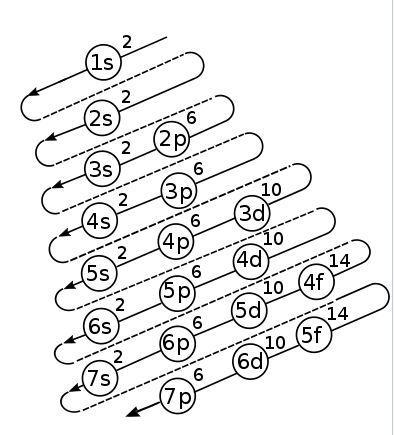
\includegraphics[width=0.2\linewidth]{figures/moeller}
	\caption{Diagrama de Moeller, las flechas indican la dirección hacia donde hay que ir para que al añadir un electrón se vaya al siguiente orbital.}
	\label{fig:moeller}
\end{figure}

Por ejemplo la configuración del sodio ($\ce{Na}, z=11$):
\begin{equation*}
	\ce{Na} (z=11): \ce{1s^{2} 2s^{2} 2p^{6} 3s^1}
\end{equation*}

A partir del último orbital se puede saber la posición del elemento en la tabla periódica, o hacer el camino inverso y averiguar la configuración electrónico a partir de la posición en la tabla. A partir de la configuración del sodio anterior podemos saber que está en $(3,1)$, es decir, en el tercer período en la primera columna. 

El número $n$ del orbital indica el período en el que se encuentra, mientra que el número $l$ (la letra) junto al superíndice, indica la columna. También con la letra del número $l$ podemos saber su posición entre los cuatro grandes grupos de la tabla periódica:
\begin{figure}[H]
	\centering
	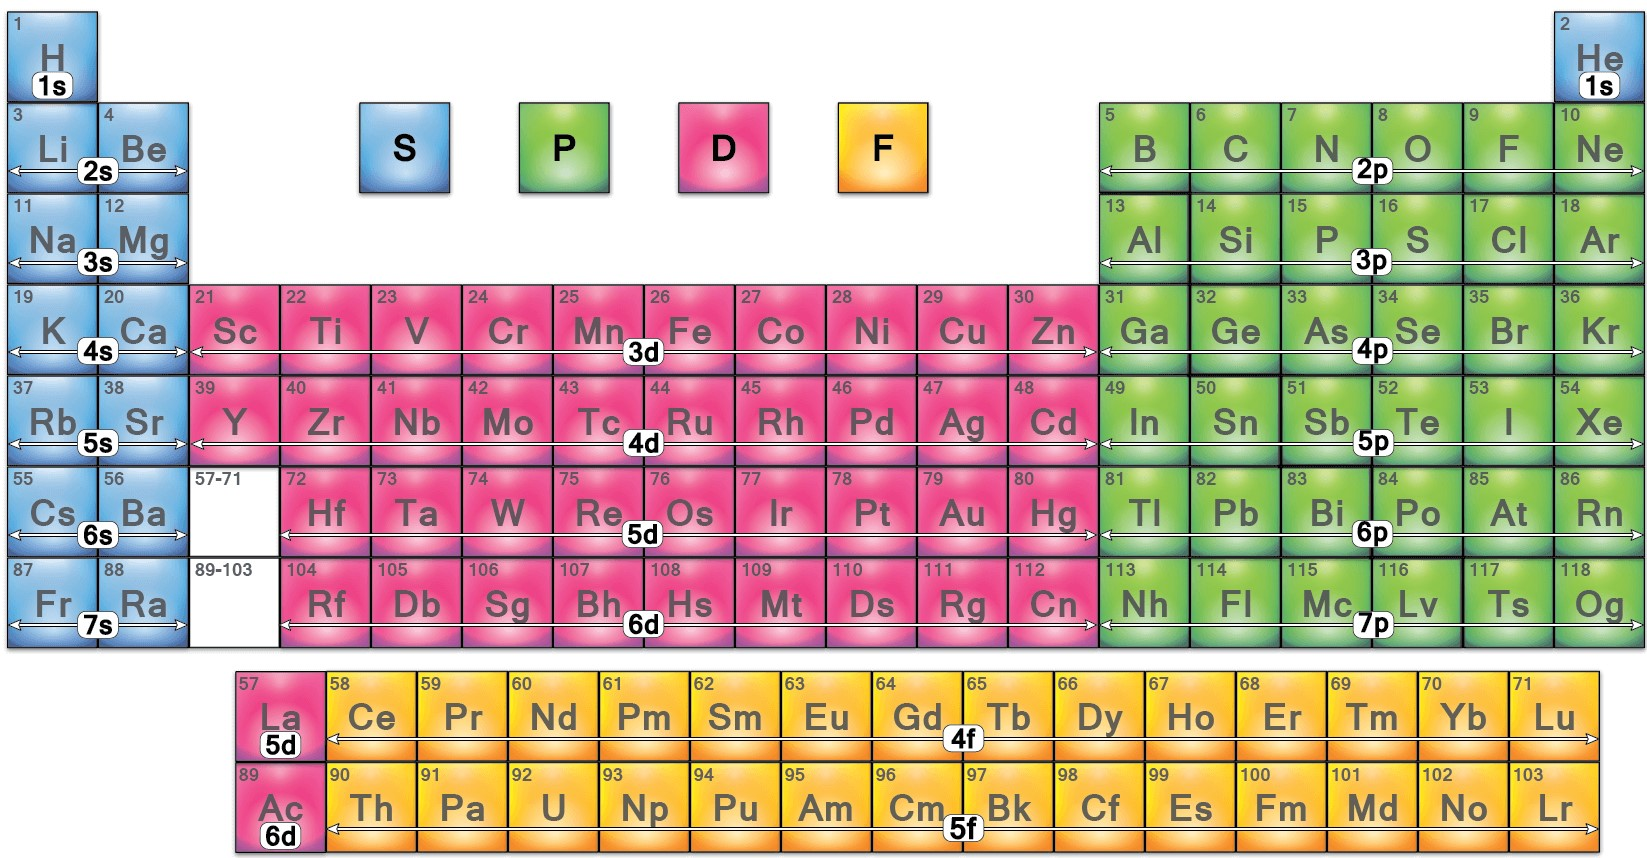
\includegraphics[width=0.8\linewidth]{figures/ptable_orbitals.png}
	\caption{Tabla periódica con la configuración electrónica de cada elemento (el último orbital). }
	\label{fig:ptableorbitalspng}
\end{figure}

\subsubsection{Periodicidad de las Propiedades de los Átomos}
Dependiendo de donde esté colocado un elemento en la tabla periódica podemos saber cualitativamente alguna de sus propiedades o lo podemos compara cualitativamente con otro elemento (decir si una propiedad es mayor o menor en relación a otro elemento). Para ello se empieza sabiendo la ubicación que tiene en la tabla periódica, usualmente en los ejercicios la posición se tiene que calcular a partir de la la configuración electrónica como ya he enseñado antes.  

Las propiedades que se pueden relacionar con la posición de la tabla periódica son las siguientes:
\begin{itemize}
	
\item \textbf{Energía Ionización $E_{i}$}:\\
Es la energía necesaria para arrancar un electrón de la capa de valencia de un átomo en estado fundamental y en fase gaseosa:
\begin{equation*}
	\ce{X_{(g)} \xrightarrow{E_{i}}}X^{+}_{(g)} + e^{-}
\end{equation*}

La cantidad de $E_{i}$ se determina a partir de estos factores:
\begin{itemize}

\item Proximidad entre el electrón y el núcleo:\\
A más proximidad (menos $n$) más $E_{i}$.

\item Carga nuclear que atrae a los electrones:\\
Cuanta más carga positiva más fuerza y más $E_{i}$.

\item Apantallamiento que hacen los electrones interior al exterior:\\
Cuanto más lejos esté un electrón más apantallamiento harán los electrones entre este y el núcleo, por lo tanto menos es la $E_{i}$.

\end{itemize}
Estos factores se pueden resumir en la ubicación del elemento de tal manera:
\begin{itemize}

\item Mismo grupo:\\
Cuanto menor sea el período (más arriba) más cerca del núcleo se encuentra y por lo tanto mayor $E_{i}$. 

\item Mismo período:\\
Dentro de un mismo período, los elementos están al mismo nivel energético y por lo tanto lo que hace variar su $E_{i}$ es cuanta carga esté en el núcleo, entonces, cuanto más a la derecha se encuentre (mayor grupo) más $E_{i}$ tendrán debido a que aumenta la cantidad de protones en el núcleo. 

\end{itemize}

Pueden haber una segunda o tercera energía de ionización, pero no será cuando se arranca un electrón de un átomo en un estado fundamental, sino un anión con carga $-1$ o $-2$, dependiendo si es la segunda o la tercera. Al saber la configuración electrónica del ion se podrá saber si su energía de ionización disminuye mucho o poco. Si al arrancar el primer electrón, no el $n$ del electrón siguiente, no habrá una gran variación en la segunda $E_{i}$. 

\item \textbf{Afinidad Electrónica}:\\
Es el cambio de energía que se produce cuando un átomo neutro en estado gaseoso captura un electrón y se forma un anión:
\begin{equation*}
	\ce{X_{(g)} + e^{-} \rightarrow X^{-}_{(g)}}
\end{equation*}
Al ser un proceso exotérmico en la muy amplia mayoría de los elementos, la afinidad electrónica suele tener signo negativo. 

Viene determinada por estos factores:
\begin{itemize}

\item La proximidad entre el electrón captado y el núcleo:\\
Cuando más cerca, más atracción y más energía se desprende en el proceso.

\item La carga nuclear:\\
Cuanta más carga (mayor $Z$) más atracción y más energía se desprende. 

\item Apantallamiento de los electrones:\\
Cuando más lejos este el electrón, más electrones de por medio y menos atracción. Este factor altera muy poco la afinidad. 
\end{itemize}

Cuando se combinan, tenemos que:
\begin{itemize}
\item Mismo grupo: \\
Cuanto más arriba (menor período), más cerca del núcleo se encuentra y menos apantallamiento hay, por lo tanto aumenta la afinidad electrónica. 

\item Mismo período: \\
Cuanto más a la derecha (mayor grupo) más carga hay en el núcleo, y más energía se libera al captar el electrón. 

\end{itemize}

\item \textbf{Electronegatividad}:\\
La electronegatividad $E_{n}$ es la forma de medir la tendencia de un átomo a atraer electrones cuando se combina formando una molécula. 

Esta propiedad no tiene unidades. Al igual que la afinidad electrónica y la energía de ionización, aumenta de abajo a arriba y de izquierda a derecha (es más fuerte arriba y a la derecha). 

Sin embargo, no aumenta de forma constante, suelen haber saltos grandes de un elemento a otro y incluso a veces disminuye en contra de la regla dicha anteriormente. El caso más notable es el hidrógeno que tiene una muy alta para estar en el primer grupo. 

\item \textbf{Energía Reticular de un Compuesto Iónico}:\\
Es la energía almacenada dentro de un compuesto iónico, se adquiere al formarlo. Es la energía que se desprende cuando se forma un mol de compuesto iónico a partir de sus iones a distancia infinita y estado gaseoso.

Este concepto se desarrollará más adelante en el tema de termodinámica. 

\item \textbf{Volumen atómico}:
Va a la par con el radio. 

\item \textbf{Radio Atómico}:
Es la mitad de la distancia entre los núcleo de dos átomos de un mismo elemento formando una molécula diátomica, una estructura covalente o estructura con enlace metálico. 

Según la posición en la tabla periódica podemos decir que:
\begin{itemize}
	
	\item Mismo Grupo:\\
	El radio aumenta de arriba a abajo (mayor período, más radio), porque aumenta el número cuántico principal, que hace aumentar la distancia del orbital al núcleo, y por lo tanto el radio. 
	
	\item Mismo Período:\\
	Va aumentando de derecha a izquierda (menor grupo, más radio), esto es porque al aumentar la carga del núcleo hay una disminución en la atracción electrón-núcleo y por lo tanto en la distancia. 
	
	Hay que decir que cuando se pasa de un elemento en estado fundamental a un ion, su radio puede cambiar debido al cambio en el número de electrones, al hacer que hayan menos (catión) hay menos repulsión entre ellos y se da lugar una contracción. Debido a que se reduce el volumen, también lo hace el radio. 
	
	En el caso de los aniones, al haber un electrón más, aumenta la repulsión entre los electrones y por lo tanto el átomo se más grande, aumentando el volumen y el radio. 
	
	La clave es pensar que los electrones se repelen entre ellos por tener la misma carga y esto afecta al tamaño del átomo. 
	
\end{itemize}


\end{itemize}



\subsection{Espectroscopia}
A través de mirar a algún tipo de espectro que surge a través de propiedades atómicas o moleculares, podemos identificar sustancias. 

\subsubsection{Espectroscopia IR}
La espectroscopia basada en la radiación infrarroja consiste en mirar el espectro de absorción de una sustancia en concreto con tal de identificarla.  

Debido a que una molécula aborde IR que tiene el efecto de cambiar su estado vibracional, podemos asociar grupos funcionales (tipos de enlaces) a picos en un espectro de transmitancia de IR de una molécula. 

En los ejercicios va a haber un gráfico parecido a este:
\begin{figure}[H]
	\centering
	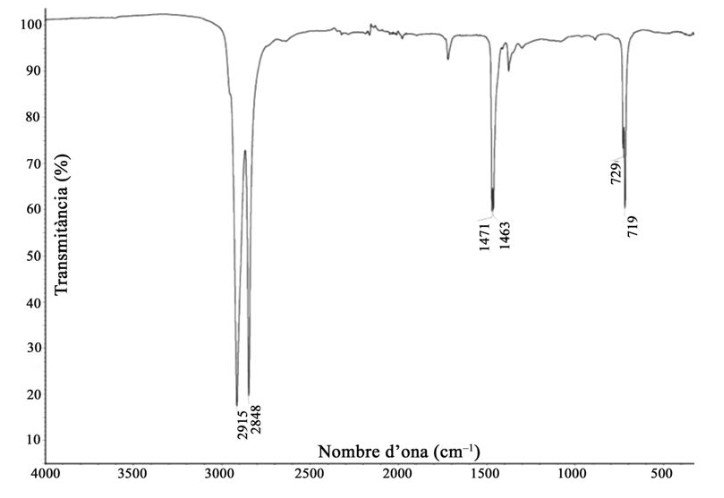
\includegraphics[width=0.5\linewidth]{figures/IR}
	\caption{Ejemplo de gráfico con espectro IR de una molécula}
	\label{fig:ir}
\end{figure}

Los picos que se pueden ver están asociados a enlaces/grupos funcionales, normalmente la correlación entre picos y enlaces se muestra mediante esta tabla:
\begin{figure}[H]
	\centering
	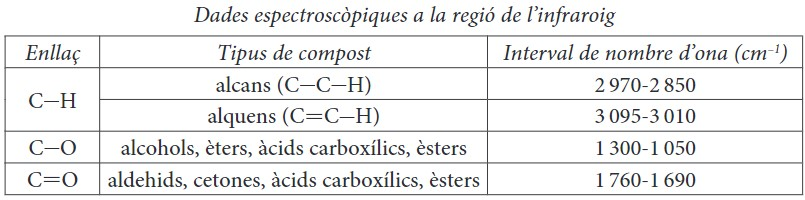
\includegraphics[width=0.7\linewidth]{figures/tabla_IR}
	\caption{Tabla en la que se muestran los enlaces y sus correspondientes picos.}
	\label{fig:tablair}
\end{figure}

Para realizar los ejercicios de este punto, hay que saber cuales son las magnitudes que se encuentran en cada eje. En el horizontal esta el número de onda $\tilde{\nu}$ que es la inversa de la longitud de onda $\tilde{\nu} = \frac{1}{\lambda}$. En el vertical está la transmitancia, el porcentaje de lo absorbido respecto a lo transmitido. Igualmente no es necesaria una definición de este concepto.  Pero si que lo es una pequeña explicación de como sucede, en la cual hay que mencionar los estados de excitación de vibración de las moléculas.  

\subsubsection{Resonancia magnética nuclear (RMN)}

Este tipo de espectroscopia funciona a partir de la orientación de los núcleos atómicos dentro de un campo magnético. Los núcleos pueden tener dos tipos de orientaciones (en sentido del campo $\vec{B}$ o en el contrario) las cuales tienen diferentes niveles de energía (estados de energía). Estos estados pueden tener transiciones entre ellos que son detectables en el campo magnético. La frecuencia de estas transiciones dependen del propio núcleo y del entorno que tiene (cantidad de enlaces). Usualmente se utiliza la RMN de protones $ \ce{H^{1}_{1}} $ la cual nos dice. 

Una RMN mide el desplazamiento químico entre un núcleo de hidrógeno respecto al patrón tetrametilsilano (TMS): 
\begin{equation*}
	\delta(\text{ppm}) = 10^{6}\frac{\nu_{\text{muestra}} - \nu_{\text{referencia}} }{\nu_{\text{referencia}} }
\end{equation*}

El desplazamiento $\delta$ está en un rango de $0$ a $12$. Es una medida que nos dice como de parecidos son los hidrógenos según su entorno. Concretamente sobre la distancia (número de enlaces) a los que están un par de hidrógenos. Aquí hay un ejemplo de un espectro con una explicación para interpretarlo:


	
	
\end{document}